% Editable native annotations around unchanged, verified IDE photographs.
\par
\begin{figure}[htbp]
\centering
\sbox0{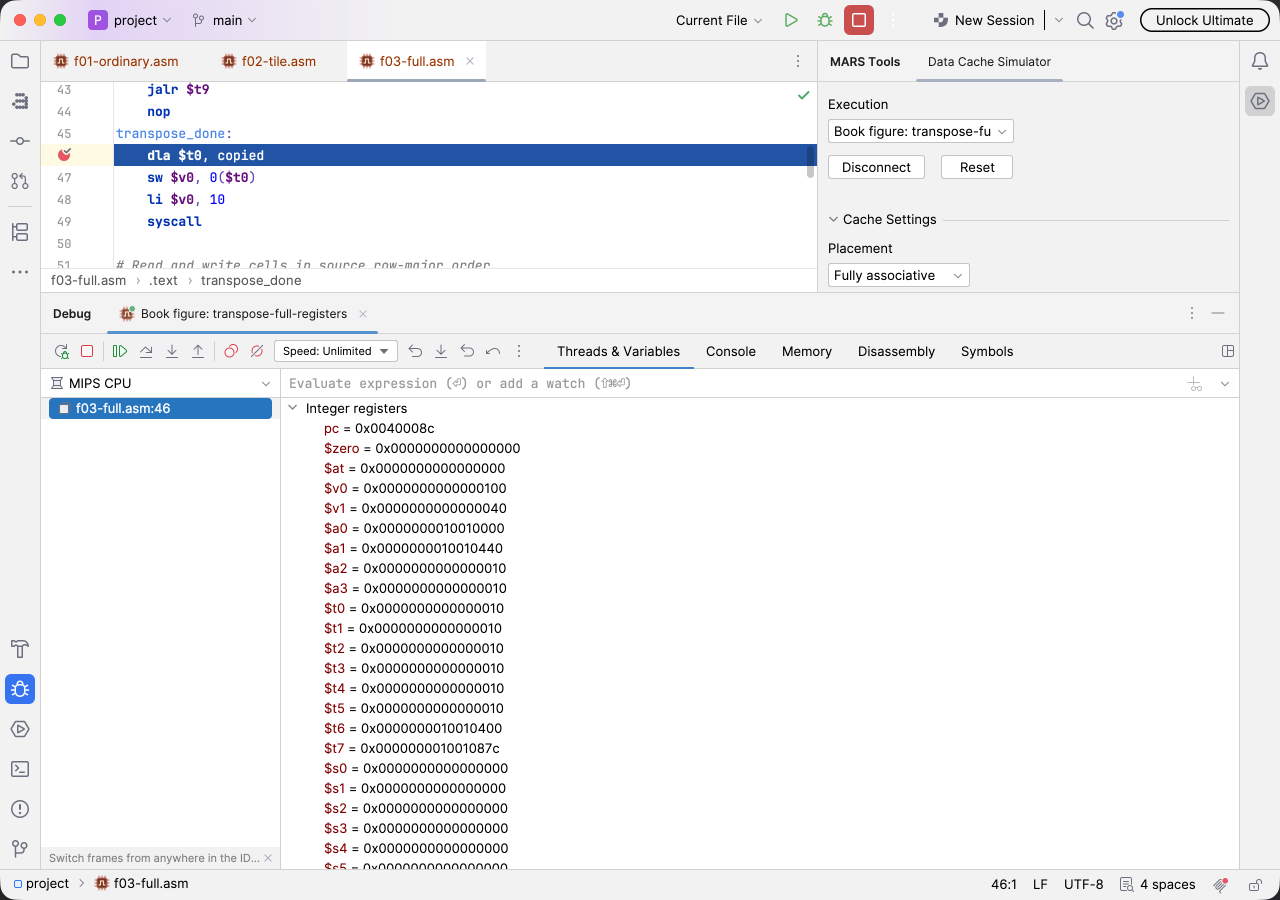
\includegraphics[artifact]{packages/011-matrix-transpose/captures/f03-full/registers.png}}
\sbox2{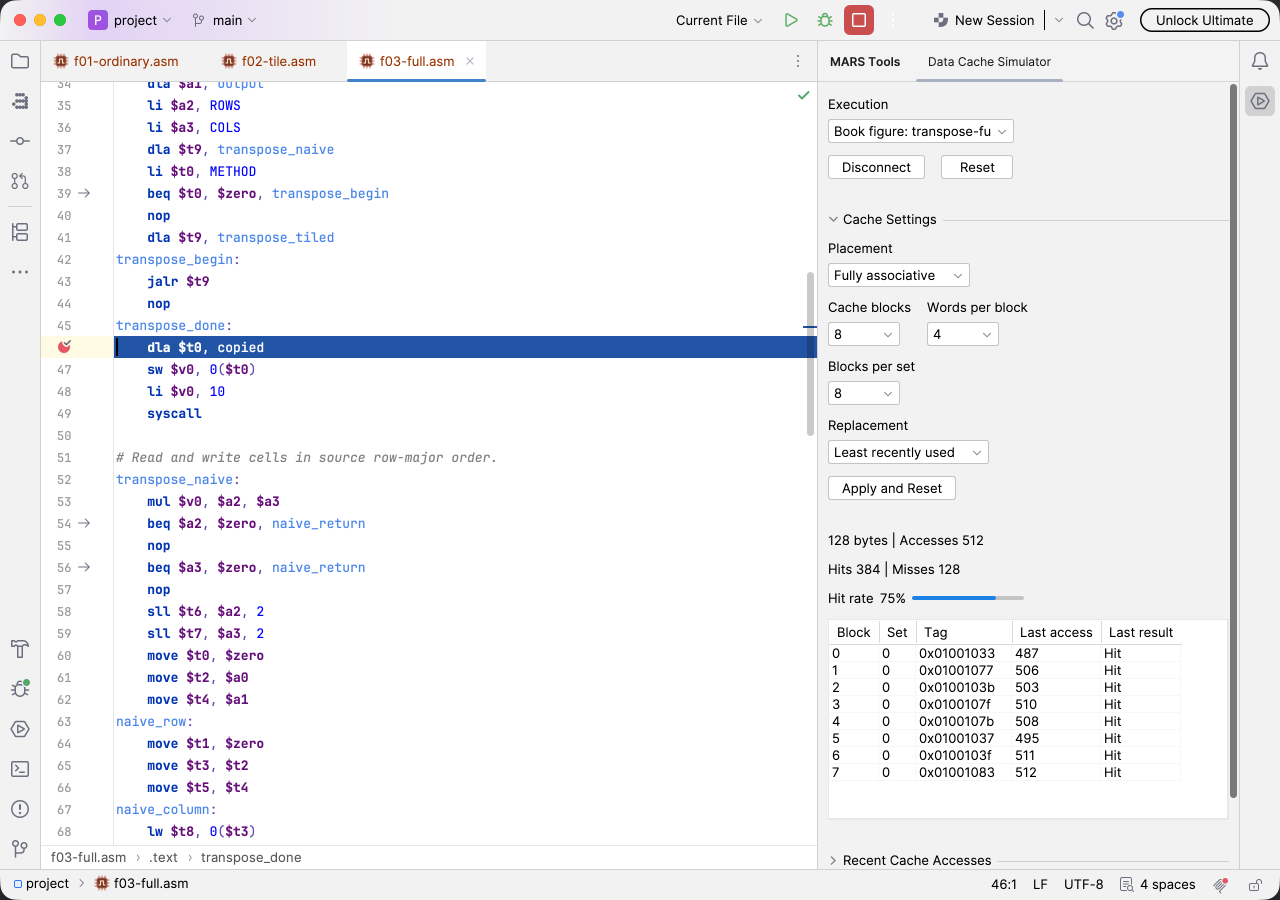
\includegraphics[artifact]{packages/011-matrix-transpose/captures/f03-full/cache.png}}
\sbox4{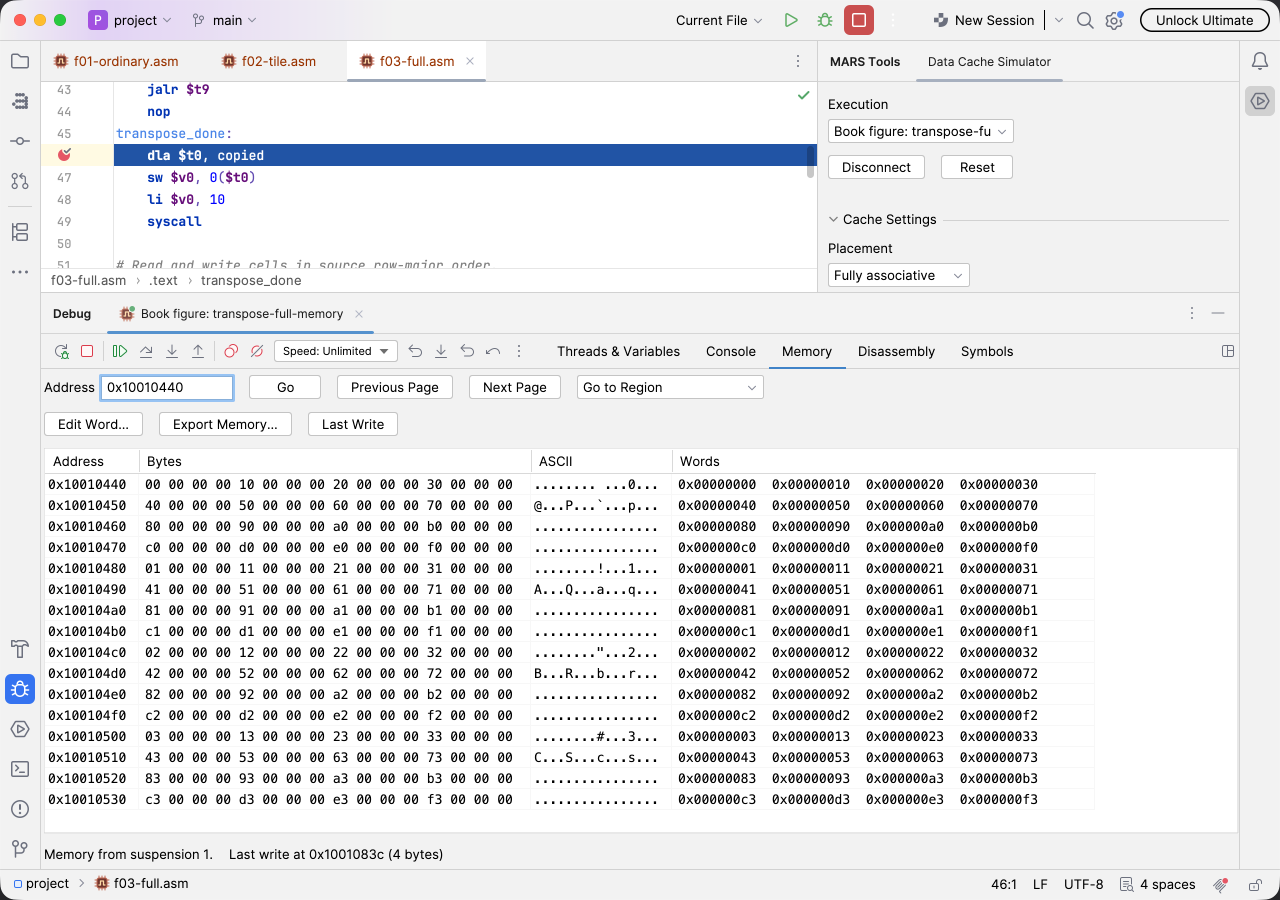
\includegraphics[artifact]{packages/011-matrix-transpose/captures/f03-full/memory.png}}
\edef\MARStransposefullsourceLeft{\the\dimexpr0.036718750\wd0\relax}
\edef\MARStransposefullsourceBottom{\the\dimexpr0.811111111\ht0\relax}
\edef\MARStransposefullsourceRight{\the\dimexpr0.713281250\wd0\relax}
\edef\MARStransposefullsourceTop{\the\dimexpr0.111111111\ht0\relax}
\edef\MARStransposefullregistersLeft{\the\dimexpr0.246093750\wd0\relax}
\edef\MARStransposefullregistersBottom{\the\dimexpr0.331111111\ht0\relax}
\edef\MARStransposefullregistersRight{\the\dimexpr0.598437500\wd0\relax}
\edef\MARStransposefullregistersTop{\the\dimexpr0.526666667\ht0\relax}
\edef\MARStransposefullgeometryLeft{\the\dimexpr0.639843750\wd2\relax}
\edef\MARStransposefullgeometryBottom{\the\dimexpr0.476666667\ht2\relax}
\edef\MARStransposefullgeometryRight{\the\dimexpr0.192187500\wd2\relax}
\edef\MARStransposefullgeometryTop{\the\dimexpr0.262222222\ht2\relax}
\edef\MARStransposefullcountersLeft{\the\dimexpr0.642187500\wd2\relax}
\edef\MARStransposefullcountersBottom{\the\dimexpr0.321111111\ht2\relax}
\edef\MARStransposefullcountersRight{\the\dimexpr0.035156250\wd2\relax}
\edef\MARStransposefullcountersTop{\the\dimexpr0.586666667\ht2\relax}
\edef\MARStransposefullmemoryLeft{\the\dimexpr0.034375000\wd4\relax}
\edef\MARStransposefullmemoryBottom{\the\dimexpr0.375555556\ht4\relax}
\edef\MARStransposefullmemoryRight{\the\dimexpr0.584375000\wd4\relax}
\edef\MARStransposefullmemoryTop{\the\dimexpr0.497777778\ht4\relax}
\begin{tikzpicture}[alt={Five annotated details after the sixteen-by-sixteen tiled routine returns. Both dimensions are hexadecimal ten, or decimal sixteen; the returned count is hexadecimal one hundred, or decimal two hundred fifty-six. The first output row is shown. Eight fully associative four-word blocks record 512 accesses, 384 hits and 128 misses, for a seventy-five percent hit rate.}]
\node[anchor=north west,inner sep=0,font=\small\bfseries] (source-title) at (6mm,0) {Next instruction};
\node[anchor=north west,inner sep=0] (source) at ([yshift=-1mm]source-title.south west) {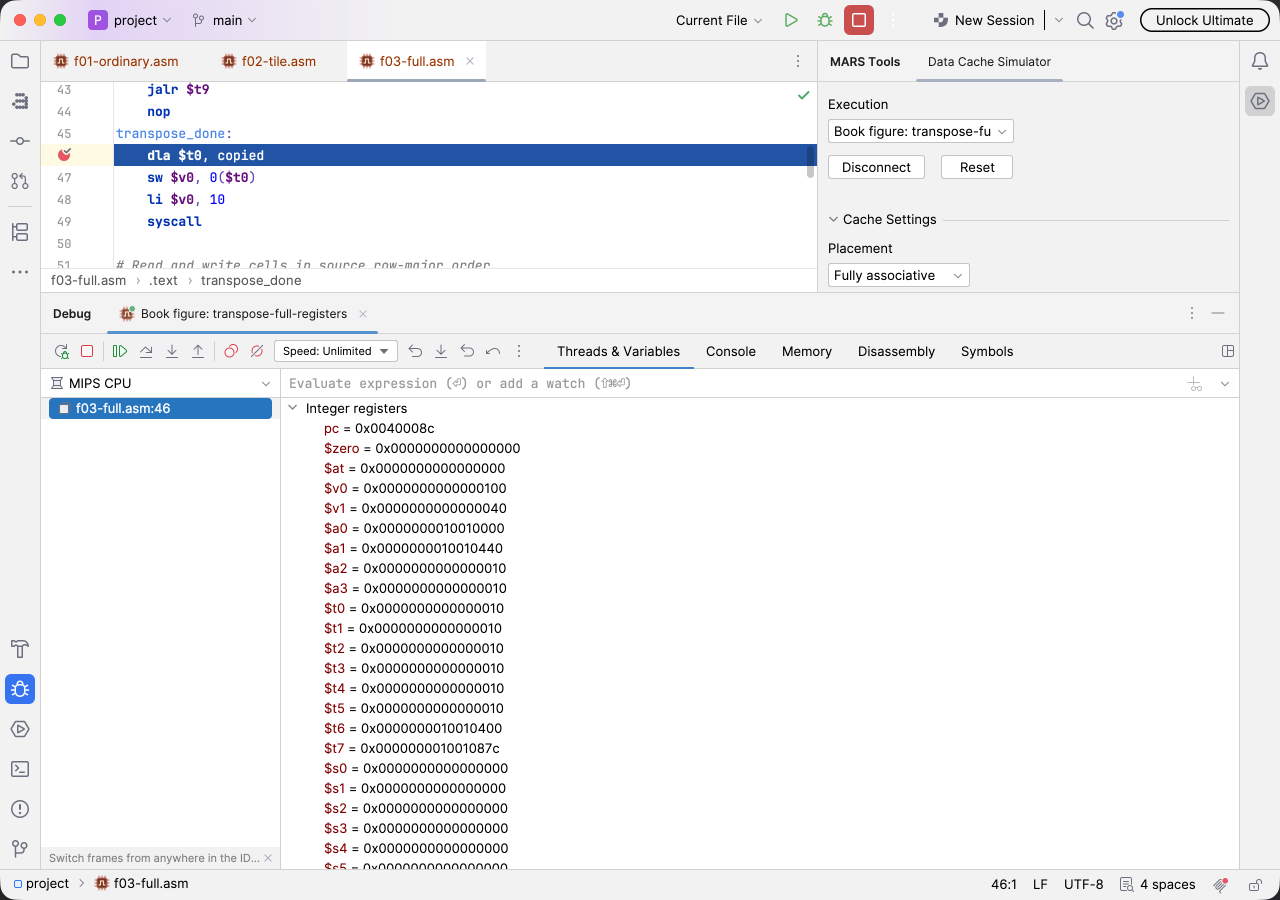
\includegraphics[width=0.5\linewidth,artifact,trim={\MARStransposefullsourceLeft{} \MARStransposefullsourceBottom{} \MARStransposefullsourceRight{} \MARStransposefullsourceTop{}},clip]{packages/011-matrix-transpose/captures/f03-full/registers.png}};
\begin{scope}[shift={(source.south west)},x={($(source.south east)-(source.south west)$)},y={($(source.north west)-(source.south west)$)}]
\draw[black,line width=0.7pt] (0.215625000,0.057142857) rectangle (0.678125000,0.371428571);
\node[draw=black,fill=white,circle,inner sep=1.5pt,font=\footnotesize] at ($(0.215625000,0.371428571)+(-3mm,0)$) {1};
\end{scope}
\node[anchor=north west,inner sep=0,font=\small\bfseries] (registers-title) at ([yshift=-2mm]source.south west) {Dimensions and count};
\node[anchor=north west,inner sep=0] (registers) at ([yshift=-1mm]registers-title.south west) {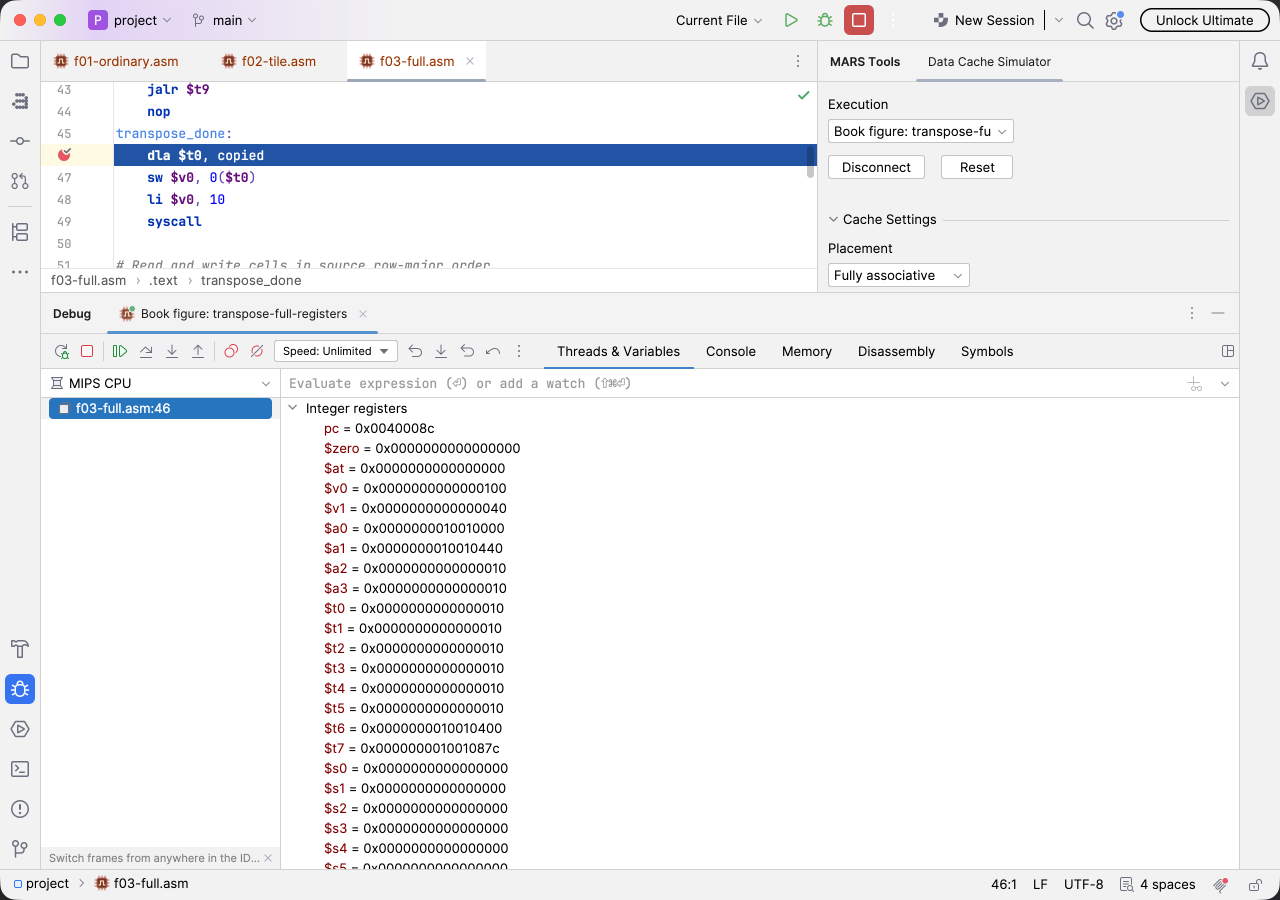
\includegraphics[width=0.33\linewidth,artifact,trim={\MARStransposefullregistersLeft{} \MARStransposefullregistersBottom{} \MARStransposefullregistersRight{} \MARStransposefullregistersTop{}},clip]{packages/011-matrix-transpose/captures/f03-full/registers.png}};
\begin{scope}[shift={(registers.south west)},x={($(registers.south east)-(registers.south west)$)},y={($(registers.north west)-(registers.south west)$)}]
\draw[black,line width=0.7pt] (0.030150754,0.031250000) rectangle (0.969849246,0.968750000);
\node[draw=black,fill=white,circle,inner sep=1.5pt,font=\footnotesize] at ($(0.030150754,0.968750000)+(-3mm,0)$) {2};
\end{scope}
\node[anchor=north west,inner sep=0,font=\small\bfseries] (geometry-title) at (0.60\linewidth,0) {Cache geometry and policy};
\node[anchor=north west,inner sep=0] (geometry) at ([yshift=-1mm]geometry-title.south west) {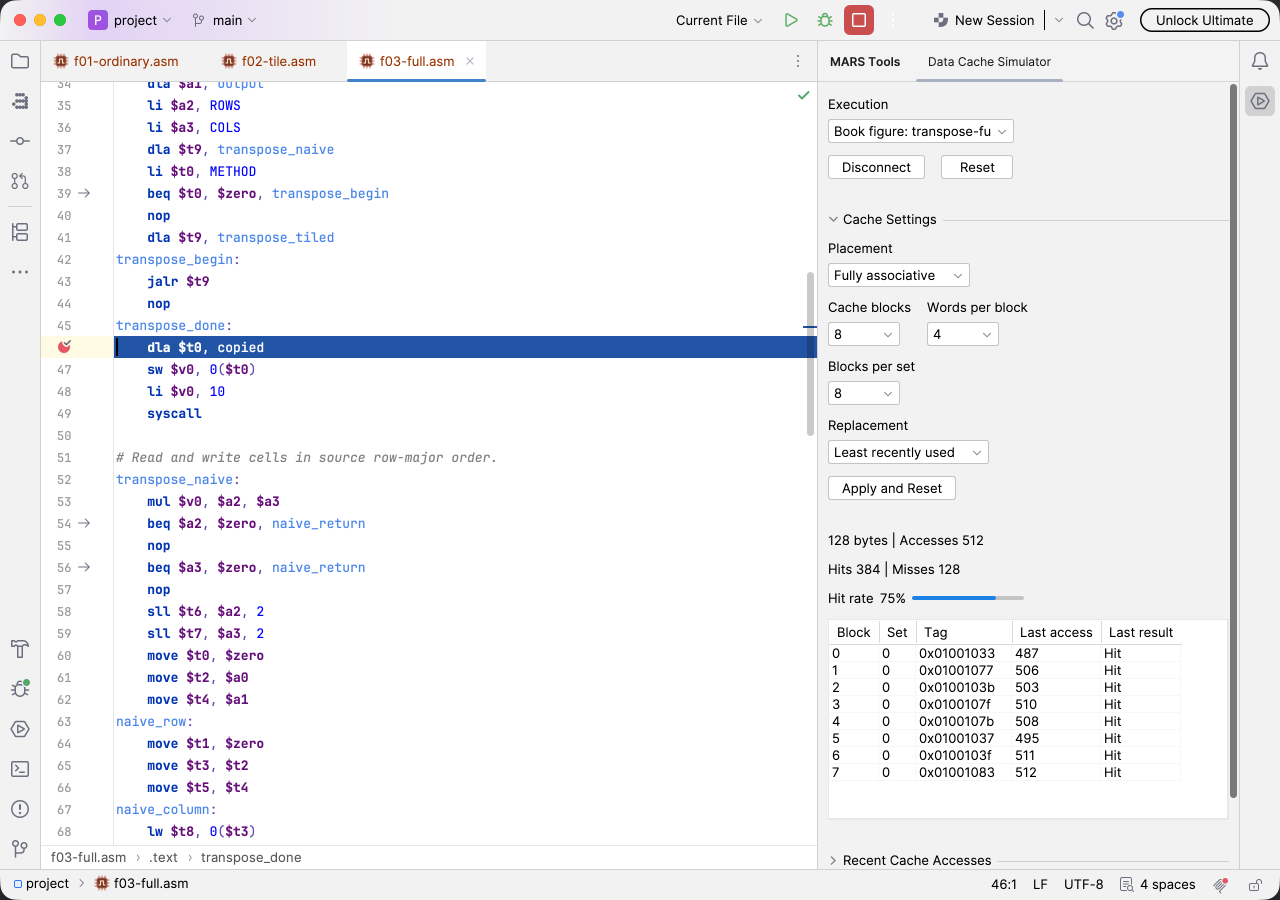
\includegraphics[width=0.31\linewidth,artifact,trim={\MARStransposefullgeometryLeft{} \MARStransposefullgeometryBottom{} \MARStransposefullgeometryRight{} \MARStransposefullgeometryTop{}},clip]{packages/011-matrix-transpose/captures/f03-full/cache.png}};
\begin{scope}[shift={(geometry.south west)},x={($(geometry.south east)-(geometry.south west)$)},y={($(geometry.north west)-(geometry.south west)$)}]
\draw[black,line width=0.7pt] (0.027906977,0.017021277) rectangle (0.972093023,0.982978723);
\node[draw=black,fill=white,circle,inner sep=1.5pt,font=\footnotesize] at ($(0.027906977,0.982978723)+(-3mm,0)$) {3};
\end{scope}
\node[anchor=north west,inner sep=0,font=\small\bfseries] (counters-title) at ([yshift=-8mm]6mm,0 |- geometry.south) {Data-access counters};
\node[anchor=north west,inner sep=0] (counters) at ([yshift=-1mm]counters-title.south west) {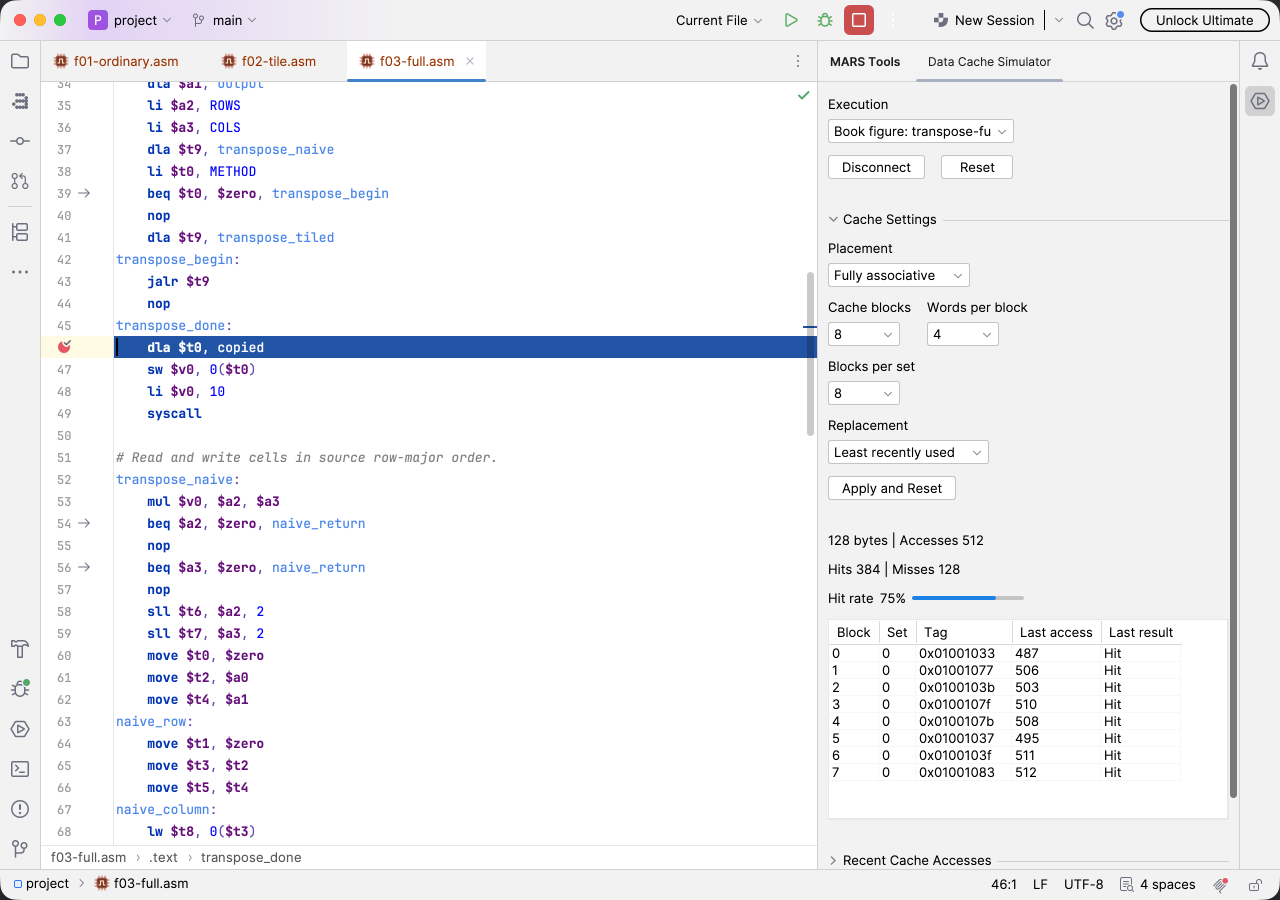
\includegraphics[width=0.60\linewidth,artifact,trim={\MARStransposefullcountersLeft{} \MARStransposefullcountersBottom{} \MARStransposefullcountersRight{} \MARStransposefullcountersTop{}},clip]{packages/011-matrix-transpose/captures/f03-full/cache.png}};
\begin{scope}[shift={(counters.south west)},x={($(counters.south east)-(counters.south west)$)},y={($(counters.north west)-(counters.south west)$)}]
\draw[black,line width=0.7pt] (0.014527845,0.048192771) rectangle (0.985472155,0.951807229);
\node[draw=black,fill=white,circle,inner sep=1.5pt,font=\footnotesize] at ($(0.014527845,0.951807229)+(-3mm,0)$) {4};
\end{scope}
\node[anchor=north west,inner sep=0,font=\small\bfseries] (memory-title) at ([yshift=-4mm]6mm,0 |- counters.south) {Output addresses and little-endian bytes};
\node[anchor=north west,inner sep=0] (memory) at ([yshift=-1mm]memory-title.south west) {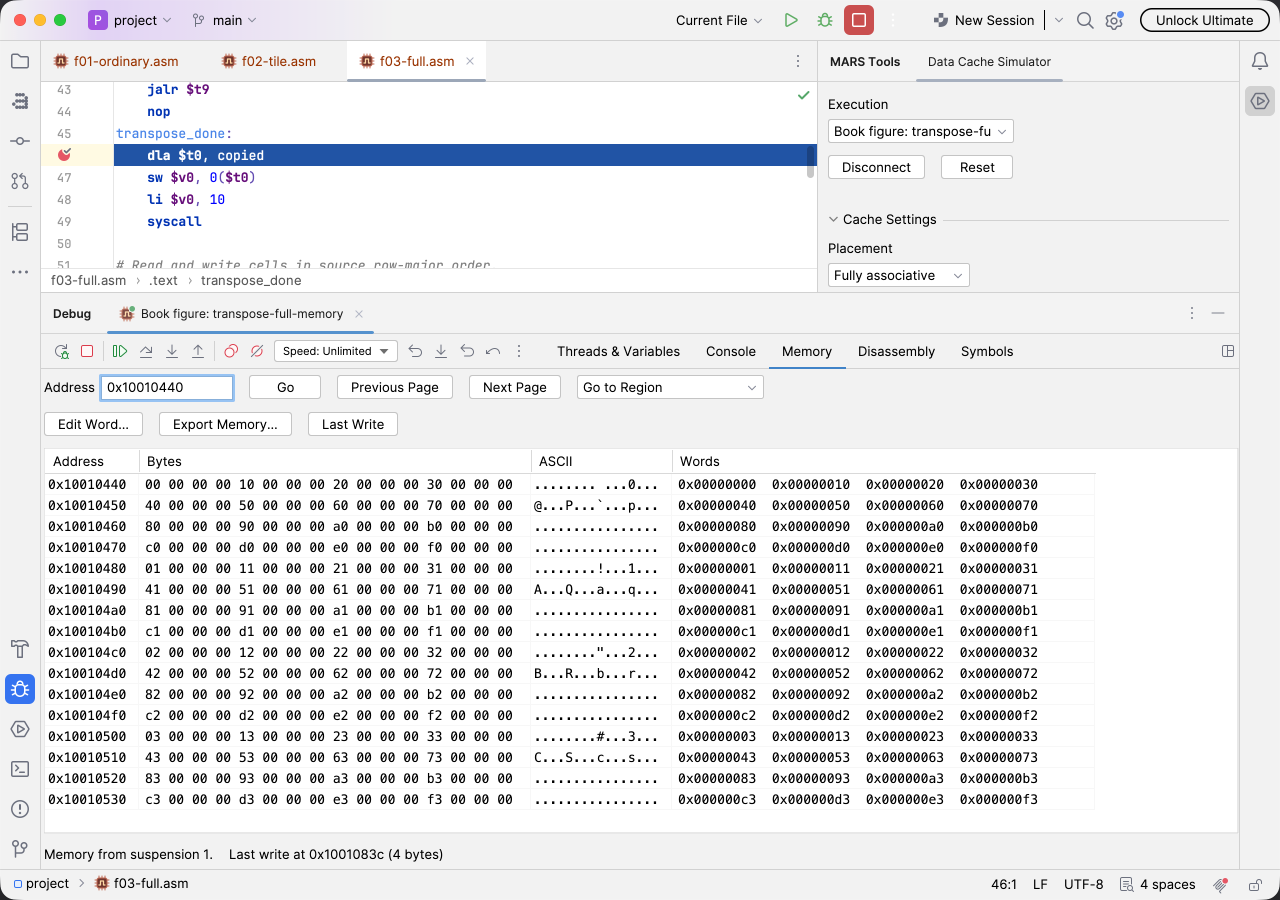
\includegraphics[width=0.78\linewidth,artifact,trim={\MARStransposefullmemoryLeft{} \MARStransposefullmemoryBottom{} \MARStransposefullmemoryRight{} \MARStransposefullmemoryTop{}},clip]{packages/011-matrix-transpose/captures/f03-full/memory.png}};
\begin{scope}[shift={(memory.south west)},x={($(memory.south east)-(memory.south west)$)},y={($(memory.north west)-(memory.south west)$)}]
\draw[black,line width=0.7pt] (0.194672131,0.035087719) rectangle (0.997950820,0.771929825);
\node[draw=black,fill=white,circle,inner sep=1.5pt,font=\footnotesize] at ($(0.194672131,0.771929825)+(-3mm,0)$) {5};
\end{scope}
\end{tikzpicture}
\par\smallskip
\begin{minipage}{\linewidth}
\small
\begin{enumerate}
\setlength{\itemsep}{2pt}
\setlength{\parsep}{0pt}
\item The stop is again before \texttt{dla \$t0, copied}. All tiles have completed and the routine has returned. The caller\textquotesingle s result store is excluded from the measured traversal.
\item Both dimension registers show \texttt{0x10}, or decimal 16. The returned \texttt{\$v0 = 0x100} is decimal 256. These are hexadecimal register values; \texttt{0x10} does not mean ten elements.
\item Eight blocks of four words still provide only 128 bytes. Fully associative placement allows any memory block in any of the eight cache blocks. The larger matrix changes the access sequence, not this cache capacity or its replacement policy.
\item Each of 256 elements causes one load and one store, giving 512 accesses. The 128 misses leave 384 hits, or exactly $75\%$. Compare these model counts with the direct-mapped run at the same return boundary.
\item The sixteen shown words form output row 0: $0,16,32,\ldots,240$. Four debugger lines make one matrix row. The complete output has 256 words; the oracle checks all of them, not just the row enlarged here.
\end{enumerate}
\end{minipage}
\caption{The completed sixteen-by-sixteen tiled transpose records 128 fully associative misses.}
\label{capture:011-matrix-transpose-f03-full}
\label{transpose-f03-full}
\end{figure}
\par
